\section{Differencing}
\label{sec:pumpkin-diff}

% TODO organize into subsections
% TODO either include some algorithm, or include a note about why not

% From Motivating the Core, modified and augmented

Differencing is aware of and guided by the semantics of Coq's rich proof term language Gallina---that is, it is a \textit{semantic differencing} algorithm.
This means that differencing can take advantage of the structure and information carried in every proof term,
thanks to Gallina's rich type theory CIC$_{\omega}$.
The rich structure of terms helps guide differencing for each configuration,
while the rich information in their types helps ensure correctness in the end.

Consider once again the example from Figure~\ref{fig:example}, but this time not just the base case.
Both versions of the proof are inductive proofs using the same induction principle, with slightly different motives.
Accordingly, differencing knows that there are two places to look for candidates, namely the base case (line 13)
and the inductive case (line 14).
Differencing breaks each inductive proof into these cases, then recursively calls itself for each case.
In the base case, it finds the candidate from Section~\ref{sec:pumpkin-spec-diff}.
Since this candidate has the desired type for the configuration specialized to the base case, differencing knows it has successfully found a candidate.

The rich type information proof terms carry helps prevent exploration of syntactic differences that are not meaningful.
For example, in the inductive case of the proof term from Figure~\ref{fig:example} (line 14), the inductive hypothesis \lstinline{IHle} changes:

\begin{lstlisting}[language=coq]
  $\ldots$ (IHle : (@\diff{n <= m0 + 1}@)) $\ldots$(@\vspace{-0.08cm}@)
  $\ldots$ (IHle : (@\diff{n <= m0}@)) $\ldots$
\end{lstlisting}
Notably, though, the type of \lstinline{IHle} changes for \emph{any} two inductive proofs over \lstinline{le}
with different conclusions. A syntactic differencing component 
may identify this change as a candidate.
My semantic differencing algorithms know that they can ignore this change.

\subsection{Design}

How differencing works in details

\subsection{Inductive Proofs as Trees}

% TODO represent inductive types by eliminators, since constructors and eliminators are dual
% TODO CIC allusion and references if possible

% From implementation

In general, the semantic differencing algorithms view inductive types as \emph{trees}.
In these trees, every node is a type context, and every edge is an extension to that type context 
with a new term.\footnote{These trees are inspired by categorical models of dependent type theory~\cite{Hofmann97}.}
Correspondingly, type differencing (to identify goal types) compares nodes, 
and term differencing (to find candidates) compares edges. 

Differencing uses these nodes and edges to prioritize semantically
relevant differences. At the lowest level, it calls a primitive differencing function 
which checks if it can substitute one term within another term to find a function between their types.

\begin{figure}[t]
\begin{center}
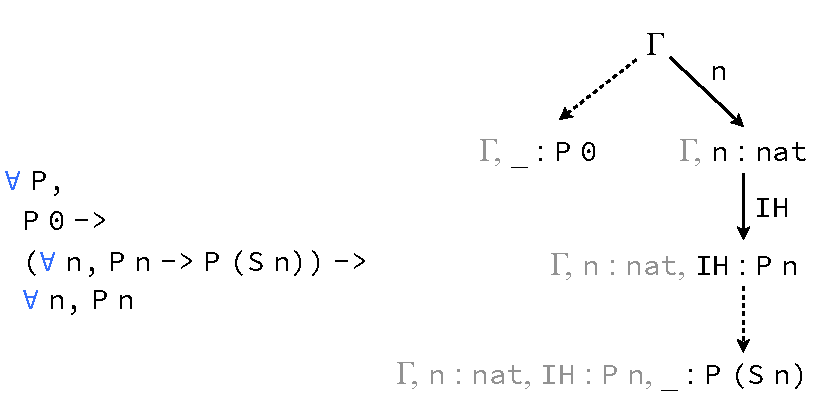
\includegraphics[scale=0.55]{repair/nat_ind}
\end{center}
\caption{The type of (left) and tree for (right) the eliminator \lstinline{nat_rect}. The solid edges represent hypotheses, and the dotted edges represent the proof obligations for each case in an inductive proof.}
\label{fig:cattree}
\end{figure}

The key benefit to this model is that it provides a natural way to express inductive proofs, so
that differencing can efficiently identify good candidates.
Consider, for example, searching for a patch between conclusions of two inductive proofs of theorems about the natural numbers:

\begin{lstlisting}[language=coq]
  nat_rect (@\diff{P}@) ... (fun (IH : (@\diff{P}@) n) => ...) : (@\ltacforall@) n, (@\diff{P}@) n(@\vspace{-0.08cm}@)
  nat_rect (@\diff{P'}@) ... (fun (IH : (@\diff{P'}@) n) => ...) : (@\ltacforall@) n, (@\diff{P'}@) n
\end{lstlisting}
In each case, differencing diffs the terms in the dotted edges of the tree for the eliminator \lstinline{nat_rect} (Figure~\ref{fig:cattree}) to
try to find a term that maps between conclusions of that case:

\begin{lstlisting}[language=coq]
  P' (@\diff{0}@) $\leftarrow$ P (@\diff{0}@)           (* base case candidate *)(@\vspace{-0.08cm}@)
  P' (@\diff{(S n)}@) $\leftarrow$ P (@\diff{(S n)}@) (* inductive case candidate *)
\end{lstlisting}
Differencing also knows that the change in the type of \lstinline{IH} is not semantically relevant (it occurs for any change in the inductive motive).
Furthermore, it knows that \lstinline{IH} cannot show up as a hypothesis in the patch,
so it attempts to remove any occurrences of \lstinline{IH} in any candidate.

When the component finds a candidate, it knows \lstinline{P'} and \lstinline{P}
as well as the arguments \lstinline{0} or \lstinline{(S n)}. This makes it simple
to query abstraction for the final patch:

\begin{lstlisting}[language=coq]
  (@\ltacforall@) (@\diff{n}@), P' (@\diff{n}@) -> P (@\diff{n}@)
\end{lstlisting}
Section~\ref{sec:pumpkin-impl-diff} describes how \sysname implements differencing.

\subsection{Limitations}

\lstset{language=coq, aboveskip=3pt,belowskip=3pt}

(Limitations and whether they're addressed in later tools yet or not.)

\paragraph{Not Fully General} Need to implement a different differencing implementation
for every kind of change, but probably should be able to abstract more.
This is mostly historical.
Later extension is able to generalize a bit more.

\begin{figure*}[ht]
\begin{minipage}{0.48\textwidth}
\begin{lstlisting}[language=coq]
fun n m p (H : n <= m) (H0 : m <= p) =>(@\vspace{-0.04cm}@)
  (@\diff{le\_S n p}@) (* ... proof of stronger lemma *)(@\vspace{-0.04cm}@)
: (@\ltacforall@) n m p, n <= m -> m <= p -> n <= (@\diff{S p}@)
\end{lstlisting}
\end{minipage}
\hfill
\begin{minipage}{0.48\textwidth}
\begin{lstlisting}[language=coq]
fun n m p (H : n <= m) (H0 : m <= p) =>(@\vspace{-0.04cm}@)
  (@\diff{le\_plus\_trans n p 1}@) (* ... proof of stronger lemma *)(@\vspace{-0.04cm}@)
: (@\ltacforall@) n m p, n <= m -> m <= p -> n <= (@\diff{p + 1}@)
\end{lstlisting}
\end{minipage}
\vspace{-.35cm}
\caption{Two proof terms \lstinline{old} (left) and \lstinline{new} (right) that contain the same proof of a stronger lemma.}
\label{fig:stronger}
\end{figure*}

\paragraph{A Challenge for Differencing} For one pair of proofs of theorems 
with propositionally equal conclusions (Figure~\ref{fig:stronger}),
the differencing component failed to find candidates in either direction.
These proofs both contain the same proof of a stronger lemma;
\sysname found patches from this lemma to
both \lstinline{old} and \lstinline{new},
but it was unable to find a patch between \lstinline{old} and \lstinline{new}.
A patch may show up deep in the difference between \lstinline{le_plus_trans}
and \lstinline{le_S}, but even if we $\delta$-reduce (unfold the definition of~\cite{equality}) \lstinline{le_plus_trans}, this is not obvious:

\begin{lstlisting}
    le_plus_trans n m p (H : n <= m) :=(@\vspace{-0.04cm}@)
      (fun lemma : m <= m + p =>(@\vspace{-0.04cm}@)
        trans_contra_inv_impl_morphism(@\vspace{-0.04cm}@)
          PreOrder_Transitive(@\vspace{-0.04cm}@)
          (m + p)(@\vspace{-0.04cm}@)
          m(@\vspace{-0.04cm}@)
          lemma)(@\vspace{-0.04cm}@)
      (le_add_r m p)(@\vspace{-0.04cm}@)
      H
\end{lstlisting}

This points to two difficulties in finding patches: Knowing when to $\delta$-reduce terms 
is difficult; exploring the appropriate time for reduction
may produce patches for pairs that \sysname currently cannot patch.
Furthermore, finding patches is more challenging
when neither theorem has a conclusion that is as strong as possible.

\paragraph{Isolating changes} Programmers sometimes make multiple changes to a verification project in the same commit;
the ideal tool should break down large changes into small, isolated changes to find patches.
This will help in finding benchmarks, supporting library and version updates, and integrating
with CI systems. We may draw on work in change and dependency management~\cite{873647, Autexier:2010:CMH:1986659.1986663, Celik:2017:IRP:3155562.3155588} to identify changes, then use the factoring component
to break these changes into smaller parts.

\paragraph{Something} \sysname has limited support for changes in hypotheses, fixpoints, constructors, 
pattern matching, and nested induction; the ideal tool should implement these features.

